% !TEX TS-program = pdflatex
% !TEX encoding = UTF-8 Unicode

% This is a simple template for a LaTeX document using the "article" class.
% See "book", "report", "letter" for other types of document.

\documentclass[11pt]{article} % use larger type; default would be 10pt

%\usepackage[utf8]{inputenc} % set input encoding (not needed with XeLaTeX)


%%% Examples of Article customizations
% These packages are optional, depending whether you want the features they provide.
% See the LaTeX Companion or other references for full information.

%%% PAGE DIMENSIONS
\usepackage{geometry} % to change the page dimensions
\geometry{a4paper} % or letterpaper (US) or a5paper or....
\geometry{margin=1in} % for example, change the margins to 2 inches all round
% \geometry{landscape} % set up the page for landscape
%   read geometry.pdf for detailed page layout information

\usepackage{graphicx} 
% \usepackage[parfill]{parskip} % Activate to begin paragraphs with an empty line rather than an indent

%%% PACKAGES
%\usepackage{booktabs} % for much better looking tables
\usepackage{array} % for better arrays (eg matrices) in maths
%\usepackage{paralist} % very flexible & customisable lists (eg. enumerate/itemize, etc.)
\usepackage{verbatim} % adds environment for commenting out blocks of text & for better verbatim
%\usepackage{subfig} % make it possible to include more than one captioned figure/table in a single float
% These packages are all incorporated in the memoir class to one degree or another...

%%% HEADERS & FOOTERS
\usepackage{fancyhdr} % This should be set AFTER setting up the page geometry
\pagestyle{fancy} % options: empty , plain , fancy
\renewcommand{\headrulewidth}{0pt} % customise the layout...
\lhead{}\chead{}\rhead{}
\lfoot{}\cfoot{\thepage}\rfoot{}

%%% SECTION TITLE APPEARANCE
%\usepackage{sectsty}
%\allsectionsfont{\sffamily\mdseries\upshape} % (See the fntguide.pdf for font help)
% (This matches ConTeXt defaults)

%%% ToC (table of contents) APPEARANCE
%\usepackage[nottoc,notlof,notlot]{tocbibind} % Put the bibliography in the ToC
%\usepackage[titles,subfigure]{tocloft} % Alter the style of the Table of Contents
%\renewcommand{\cftsecfont}{\rmfamily\mdseries\upshape}
%\renewcommand{\cftsecpagefont}{\rmfamily\mdseries\upshape} % No bold!

%\usepackage[T1]{fontenc}
\usepackage[latin9]{inputenc}
%\usepackage[active]{srcltx}
\usepackage{setspace}
\doublespacing
\usepackage[english]{babel}

\begin{document}

\title{Connectivity Analysis of Metagenomic Data}
\author{ACH, JP, RCK, RM, JJ, JMT, CTB}
\maketitle

\section{Introduction}
Given the rapid decrease in the costs of sequencing, we can now achieve the sequencing depth necessary to study even the most complex environments \cite{Hess:2011p686,Qin:2010p189}.  The main bottleneck for these metagenomic studies is the lack of effective strategies to annotate and predict gene functions from the enormous sequencing datasets that are now being generated \cite{Hoff:2009p913,Kunin:2008p16,Noguchi:2006p968,Zhang:2012p959}.  De novo metagenomic assembly has been used as a solution to reduce dataset size by collapsing numerous short reads into fewer contigs and providing longer sequences containing multiple genes and operons \cite{Miller:2010p226,Pop:2009p798}.  Furthermore, because it does not rely on the availability of reference genomes, assembly also produces novel contigs allowing for comparisons of sequences within and between metagenomes \cite{Li:2009p707,Schloss:2008p2} or annotations of unknown genomes \cite{Hess:2011p686}.  The success of de novo metagenomic assembly relies on the ability to store information about the connectivity of sequencing reads within an assembly graph.  Thus, its application to large and complex metagenomic datasets is limited by both the amount of sequencing and the availability of computational memory. 

To deal with these challenges, new metagenome-specific de novo assemblers use various "divide and conquer" approaches to break apart components of the assembly graph \cite{Peng:2011p898} (cite metaVelvet).  These assemblers take advantage of the fact that environmental populations contain multiple genomes which have been sampled at varying depths corresponding to their natural abundance.  Read coverage (the extent to which sequencing reads contribute to assembled contigs) and/or graph connectivity are used to break apart and simplify metagenomic assembly graphs. 

The ability to resolve components of an assembly graph depends on accurately distinguishing variable-coverage genome sequences from sequencing errors and bias.  The presence of sequencing biases and errors have been demonstrated in Illumina sequences \cite{Harismendy:2009p228,Hoffmann:2009p1027,Nakamura:2011p741} but very little is known about their effects on assembly graph properties and the resulting assemblies.  With large amounts of sequencing (as is needed for complex metagenomes), increases in the number of real biological sequences are accompanied by increases in sequencing errors and biases.  In this study, we analyzed the ability to resolve disconnected components of several metagenomic assembly graphs.  In doing so, we identified highly-connecting sequences in several metagenomes which we demonstrate originate from sequencing artifacts.  We evaluated the effects of removing these sequences on metagenomic assembly and discuss how this approach ultimately enables the assembly of large, complex metagenomes.  

\section{Results}

\subsection{Connectivity analysis of metagenome datasets}

\subsubsection{Presence of a single, highly-connected lump in all datasets}
We selected datasets from three diverse, medium to high complexity metagenomes from the human gut \cite{Qin:2010p189}, cow rumen \cite{Hess:2011p686}, and agricultural soil (unpublished) (Table 1). We also included one simulated metagenome (error-free) of a high complexity, high coverage (\textasciitilde{}10x) microbial community \cite{Pignatelli:2011p742}. To study the effects of increased sequencing, we also included two additional subsets of the agricultural soil metagenome containing 50 million and 100 million reads each.   The coverage of each metagenome was estimated by aligning reads to corresponding assembled contigs (see Methods).  The read coverage of the selected metagenomes ranged from 1 to 32\%.   For the human gut and cow rumen metagenomes, we estimate 32.4\% and 3.5\%, respectively.  For the small, medium, and large soil metagenomes, the coverage was estimated at 1.4\%, 4.7\%, and 5.60\%, respectively (Table X).  

The connectivity of reads within the assembly graph of each dataset was evaluated within a de Bruijn graph representation (see Methods).  Reads contributing to disconnected portions of the assembly graph were separated.  In each dataset, we identified a dominant, highly-connected set of sequencing reads which we referred to as the "lump" (Figure 1, Table 1).  In the simulated dataset, this lump consisted of 5\% of the reads.  In the metagenomes, the size of the lump ranged from 7\% (in the smallest soil metagenome) to 67\% (in the human gut metagenome) of the total reads.  For the three soil datasets of increasing size, the size of the lump was disproportionately larger than the increase in sequencing (Figure 1, Table 1).  As the number of reads increased by 2-fold and 5-fold, the size of the lump increased by 5-fold and 14-fold, respectively.  

@AC - I chose to just leave this out but FYI...  In a smaller subset of the human gut metagenome (50 million reads), the relative size of the lump was similar and comprised over 75\% of the sequencing reads (data not shown). 

\begin{figure}
\center{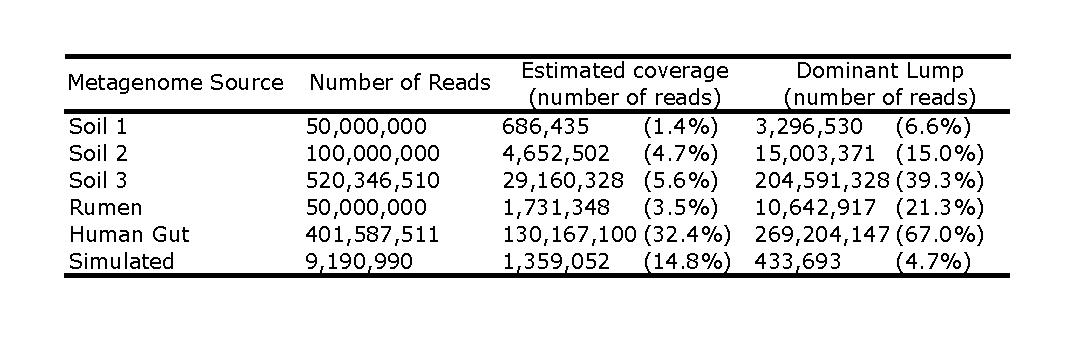
\includegraphics[width=5in]{./figures/table1.pdf}}
\caption{The connectivity of sequencing reads from medium to high complexity metagenomes from the soil, rumen, and human-gut were analyzed.  Read coverage was estimated by aligning sequencing reads to Velvet-assembled contigs (K=33).  A dominant lump, or largest disconnected component of each metagenome assembly graph, was identified in each metagenome. }
\end{figure}

\begin{figure}
\center{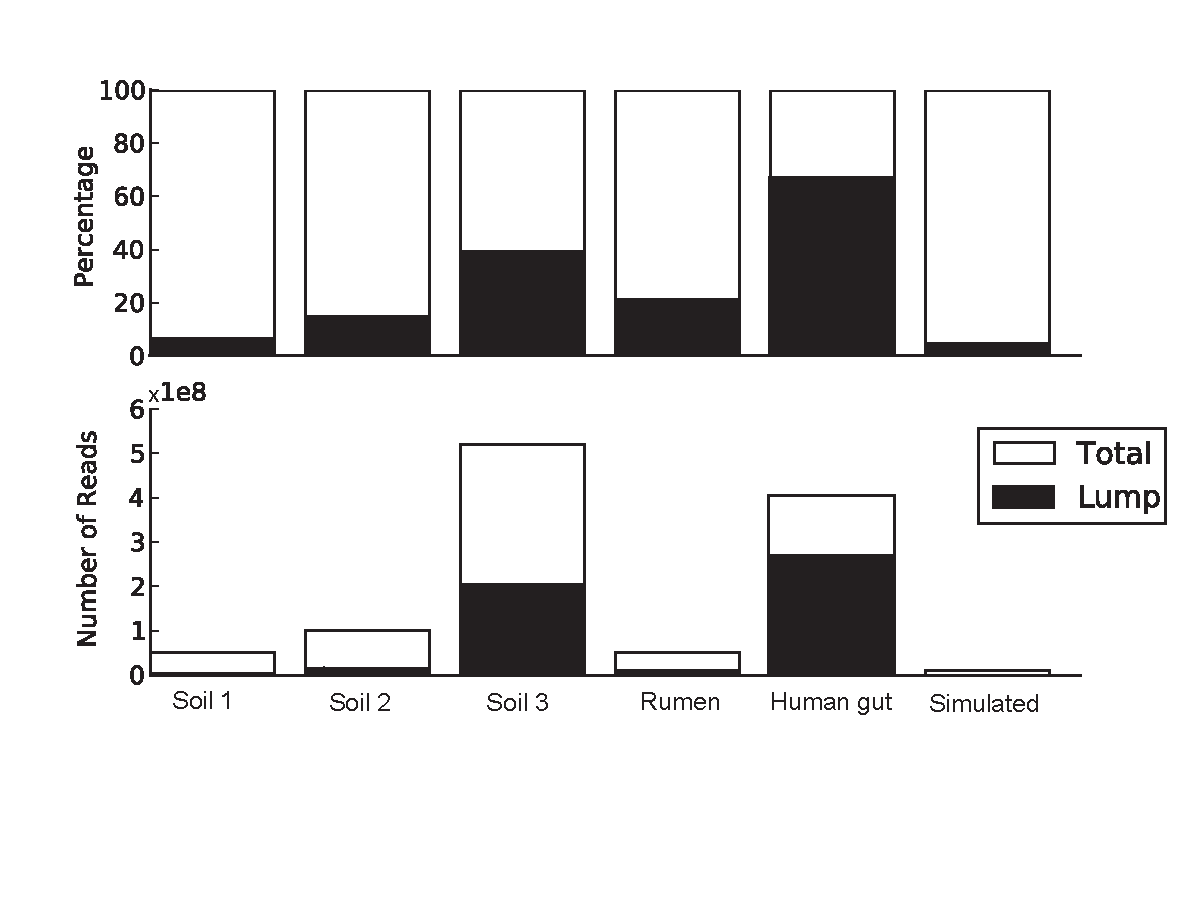
\includegraphics[width=5in]{./figures/lump_sizes.pdf}}
\caption{The presence of a dominant lump was identified for all metagenomes studied, regardless of origin of the metagenome.}
\end{figure}

@Note that filtering out highly abundant k-mers effects - CTB, need to analyze...need to ask question about this

\subsubsection{Characterizing assembly graphs in metagenomic and simulated lumps}

To assess the degree of connectivity of sequences within the lump, we measured the local graph density of reads within the de Bruijn assembly graph of each metagenome (Table X).  The local graph density is defined here as the number of k-mers, or sequences of length k, found within a distance of N divided by N.  Examining the connectivity of all 112 bacterial genomes used for the simulated dataset, we found that fewer than 2\% of the nodes within the assembly graph had an average graph density greater than 20.   The simulated short reads generated from these genomes resulted in a lump made up of 4.7\% of total reads.  Within this lump, 17\% of the nodes had an average graph density greater than 20.  Similarly, in lumps from metagenome datasets, average graph density greater than 20 ranged from 21 to 50\%.  

\begin{figure}
\center{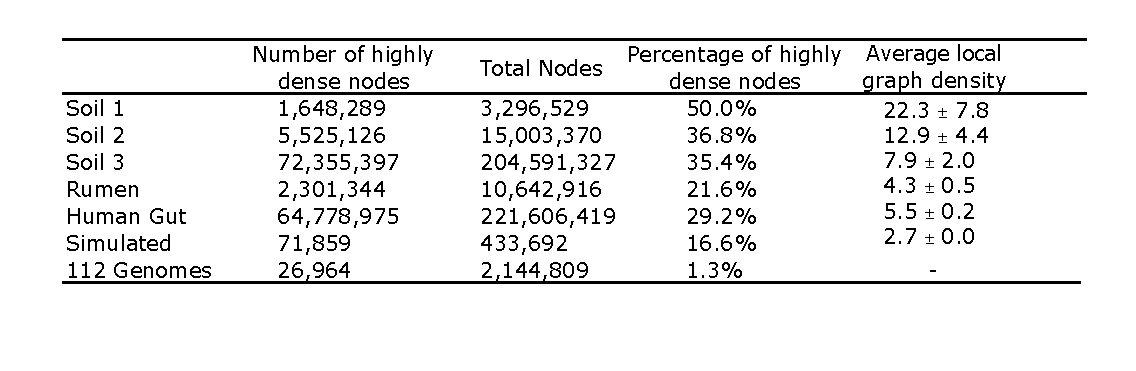
\includegraphics[width=5in]{./figures/density_table.pdf}}
\caption{The number of highly dense k-mer nodes with local assembly graph densities greater than 20 (N=100) for various metagenomes and a mixture of 112 reference genomes \cite{Pignatelli:2011p742}. For the human gut metagenome, partial traversal of the graph (82\%) was used to calculate the number of highly dense nodes due to computational limitations.  The local graph density (N=10) for all nodes in each metagenome was calculated for each k-mer position within reads (see Figure X), and the average density for all k-mer positions is shown.}  
\end{figure}

We next determined the extent to which graph density varied by position along sequenced reads by measuring the average local graph density within ten steps of every k-mer by position in a read (Figure 2).  For the simulated dataset, the average local density was stable for all positions along reads.  In contrast, metagenome datasets had increased average local graph densities which varied depending on read position.  The reads in the lumps in the soil metagenomes had the most variability of local graph densities by position, with standard deviations ranging from 25\% - 35\% of the average density, and increases in density occurred at the 3' end end of the read.

@is this a real number that people usually report, % of standard deviations, there's probably a better way to say this

\begin{figure}
\center{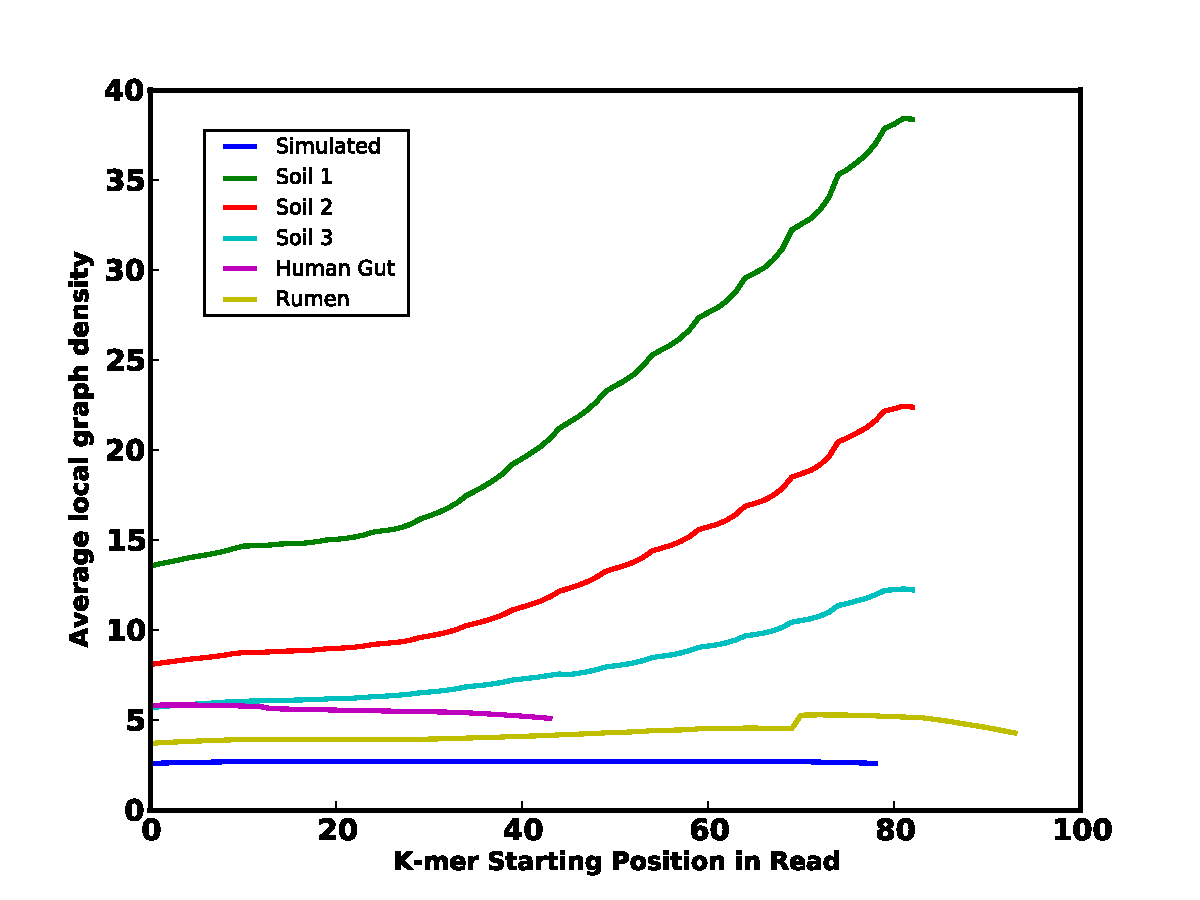
\includegraphics[width=5in]{./figures/density_pos.pdf}}
\caption{The extent to which average local graph density varies by read position is shown for the lump of various datasets.  Unlike the graph density of the simulated metagenome lump, average graph density of sequences in metagenomic lumps varied significantly by position along the read.}
\end{figure}

\subsection{Identification of highly-connecting k-mers and their effects on assembly}

\subsubsection{Characteristics of highly-connecting sequences in simulated and metagenomic lump reads}

We next identified sequences within each lump which were causes of high local graph density using a systematic assembly graph traveral algorithm (see Methods).  For sequences within the lumps of metagenomic datasets, we found that 6 to 8\% of the unique k-mers were highly-connective, with the exception of the smallest soil metagenome lump which contained less than 1\% of highly-connective k-mers.  In contrast, the lump of the simulated metagenome contained fewer of these highly connective k-mers, 3\% of total unique k-mers (Table X).  

Having identified these highly-connective sequences, we next assessed the extent to which these k-mers were found at specific positions along a sequencing read (Figure X).  In the simulated metagenome lump, the highly-connecting k-mers did not exhibit any bias with regard to position within the read.  In other words, these k-mers had equal probability of being located at any position along the read.  In the case of metagenome lumps, highly connective k-mers were more prevalent at position-specific locations along the read (Figure X).   For the three soil metagenomes, the fraction of total k-mers which were identified as highly-connective increased at the 3'-end of the read.  In the human-gut and rumen metagenome lumps, the fraction of these k-mers decreased at the 3'-end of the read.    

\begin{figure}
\center{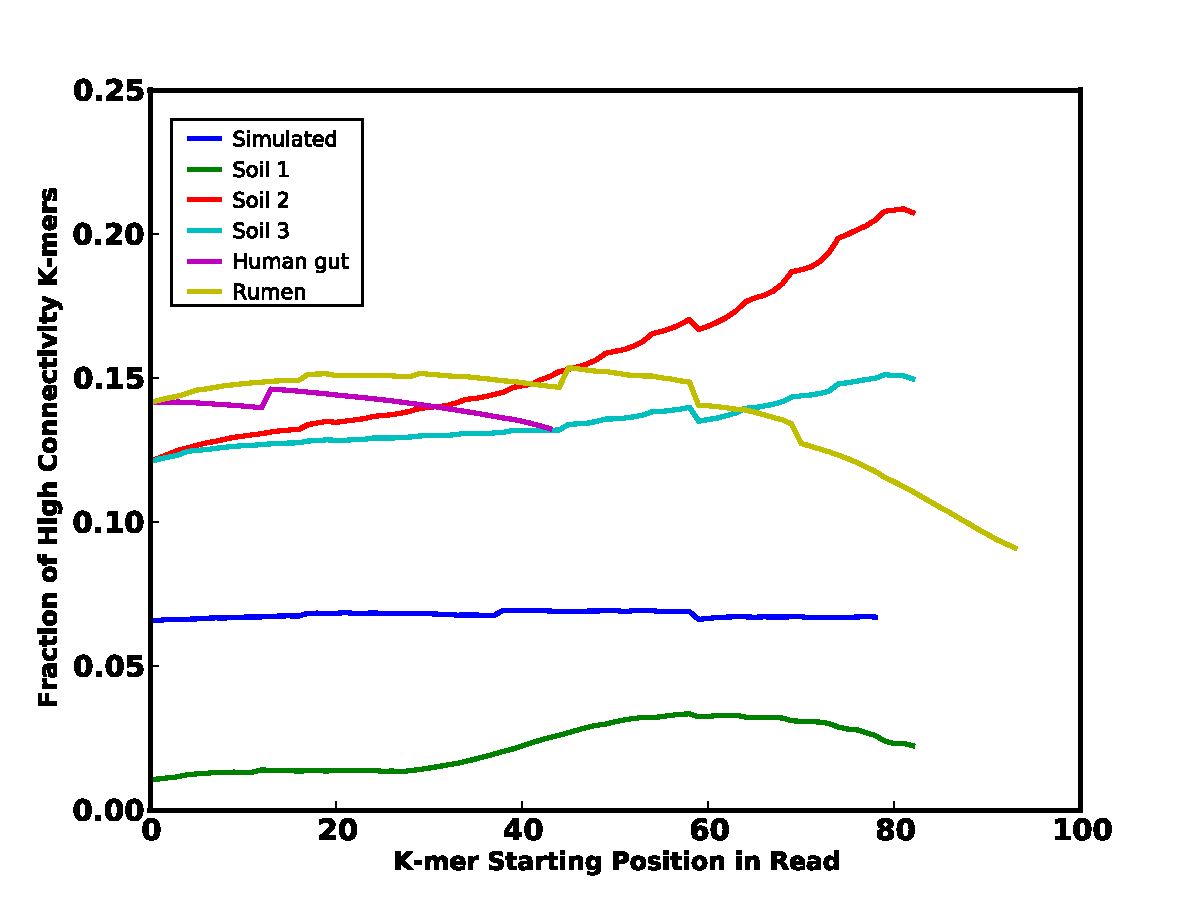
\includegraphics[width=5in]{./figures/position_read.pdf}}
\caption{The extent to which highly-connecting k-mers are present at specific positions within sequencing reads for various metagenomes.}
\end{figure}


\subsubsection{Characteristics of highly-connecting sequences in simulated and metagenomic lump assemblies}

We were interested in the incorporation of the highly-connective k-mers in the final assembly of the sequences within the lumps.  For all lumps, we found that the there was an enriched presence of these k-mers within reads compared to the final assembly (Table X).  In the simulated lump, there was an 6-fold enrichment of these sequences in the reads compared to the assembled contigs.  Likewise, in metagenomic lumps, there was a 3 to 6 time enrichment of highly-connective k-mers in reads over the assemblies.  Examining the position of these highly-connecting k-mers within assembled contigs, we found that these sequences were being disproportionately placed on the ends of contigs (Figure X) in every metagenome assembly studied.  


\begin{figure}
\center{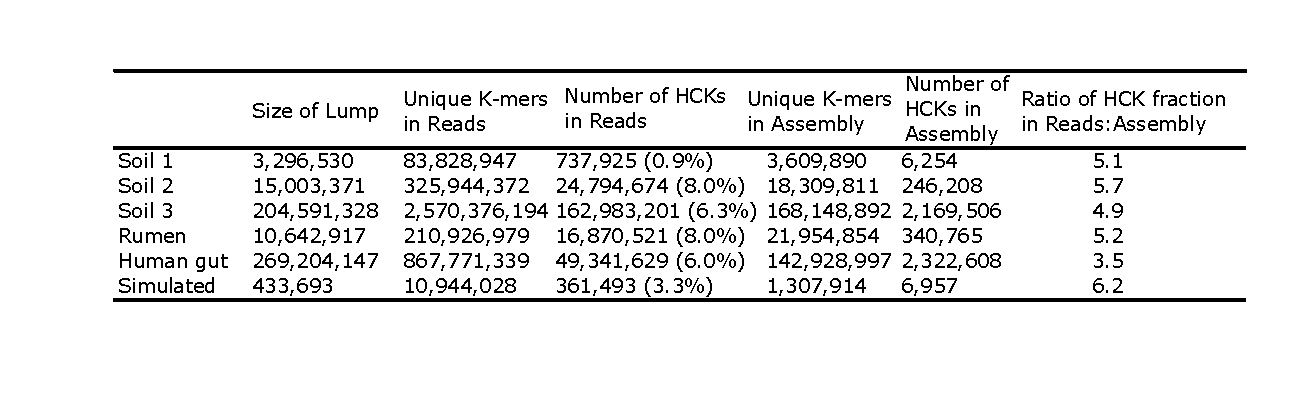
\includegraphics[width=5in]{./figures/stoptag_table.pdf}}
\caption{Highly-connecting k-mers were more highly enriched in sequencing reads compared to assembled contigs.  All metagenomes (except for the soil 3 and human gut) were assembled with Velvet (as described in Methods) with K=25, 27, 29, 31, 33 and merged.  Enrichment ratios for soil 3 and human gut metagenomes calcuated from assemblies at only at K=33 due to computational limitations.}
\end{figure}

\begin{figure}
\center{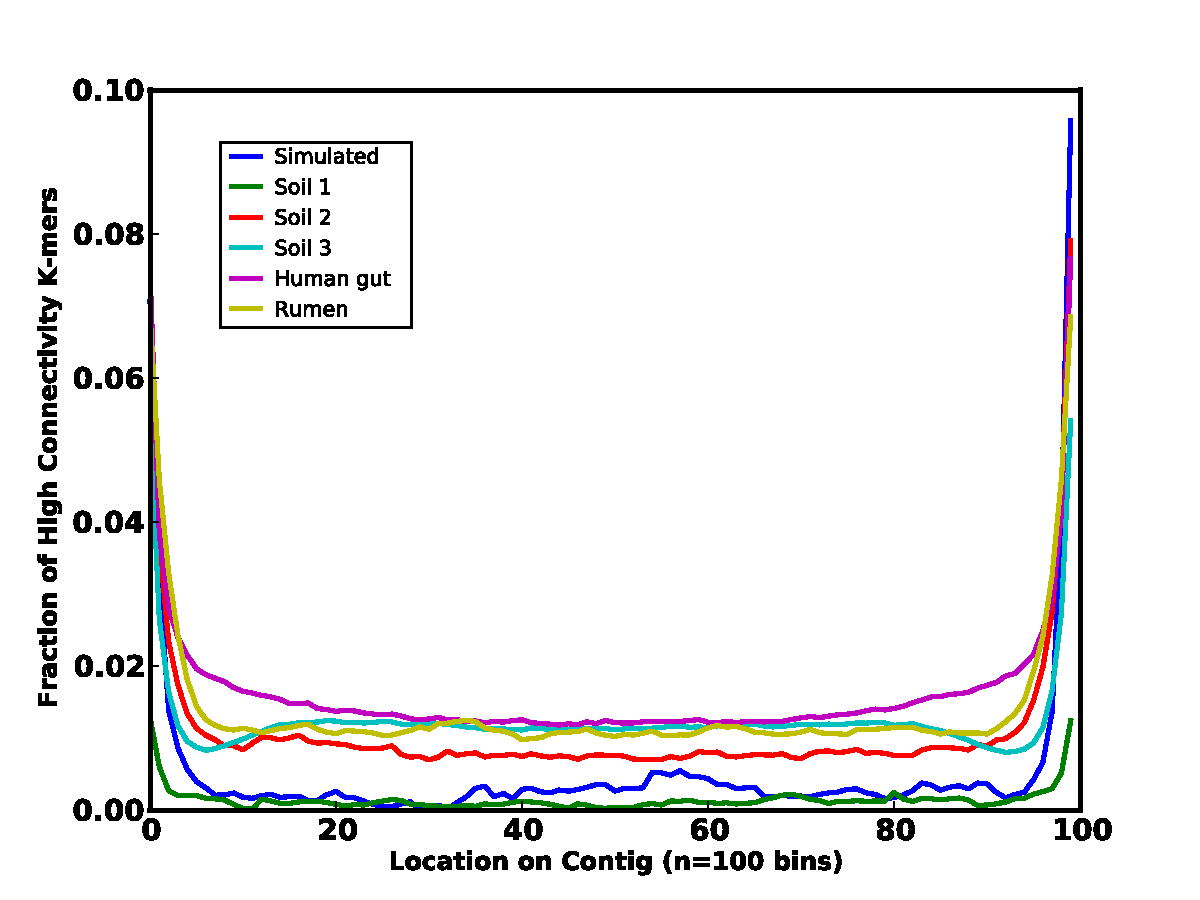
\includegraphics[width=5in]{./figures/pos-spec-bias-contigs.pdf}}
\caption{When incorporated into an assembly, highly-connecting sequences (k-mers) were disproportionately present at the ends of contigs.}
\end{figure}

\subsection{Effects of removal of highly-connecting k-mers on assembly}

\subsubsection{Effects of removing highly-connecting k-mers on the simulated lump assembly}
To study the effects of the highly-connecting k-mers on assembly, we performed assemblies of the simulated metagenome lump with and without removal of the identified highly-connective k-mers from reads.  As a result of removing these sequences, several assembly statistics improved.  Whereas the unfiltered assembly contained 1,844 contigs (maximum size = 3,787 bp) with 1,365,436 bp, the filtered assembly contained 2,301 contigs (maximum size = 5,826 bp) with 1,733,645 bp (Table X).  Overall, we estimate the unfiltered and filtered assemblies to be quite different.  Based on comparing constituent k-mer composition, we estimate the assemblies to 69\% similar.  Of the 1,844 contigs in the unfiltered assembly, we estimate that 375 (20\%) are unique.  In the filtered assembly, we estimate that 1,136 of the 2,301 contigs (49\%) are unique (Table X). 
	We next identified protein coding regions from the assemblies by predicting open reading frames (ORFs) from assembled contigs with lengths greater than 500 bp (see Methods).  The filtered assembly contained more ORFs compared to the unfiltered assembly, 3,049 filtered ORFs and 2,401 unfiltered ORFs (Table X).  To evaluate the accuracy of each assembly, we compared the predicted ORFs to the original 112 genomes which were used to generate the simulated metagenome.  In the unfiltered assembly, 2,395 (99.8\%) ORFs matched the reference genomes while in the filtered lump assembly, more assembled ORFs, 3,037 (99.6\%), matched the reference genomes.  Overall, the unfiltered and filtered assemblies shared shared a total of 2,018 ORFs which varied in lengths between unfiltered and filtered assemblies.  Comparing the alignment length of predicted ORFs to reference proteins, we found that the filtered assembly had slightly longer ORF alignment lengths compared to the unfiltered assembly (460 ORFs), and few ORFs had longer alignments in the unfiltered assembly (402 ORFs).  The large majority of shared ORFs had no difference in alignment lengths (1,156 ORFs) (Figure X).  

@@are the unique orfs shorter? - small signal, not sure if good enough if strong enough to include here, decided to leave this out
@ Note that I left out the edge effects of ORFs...I thought it was just too funky and vague.  I think the annotations against the references make for the stronger argument.  We can put it back in though if you like it.

\begin{figure}
\center{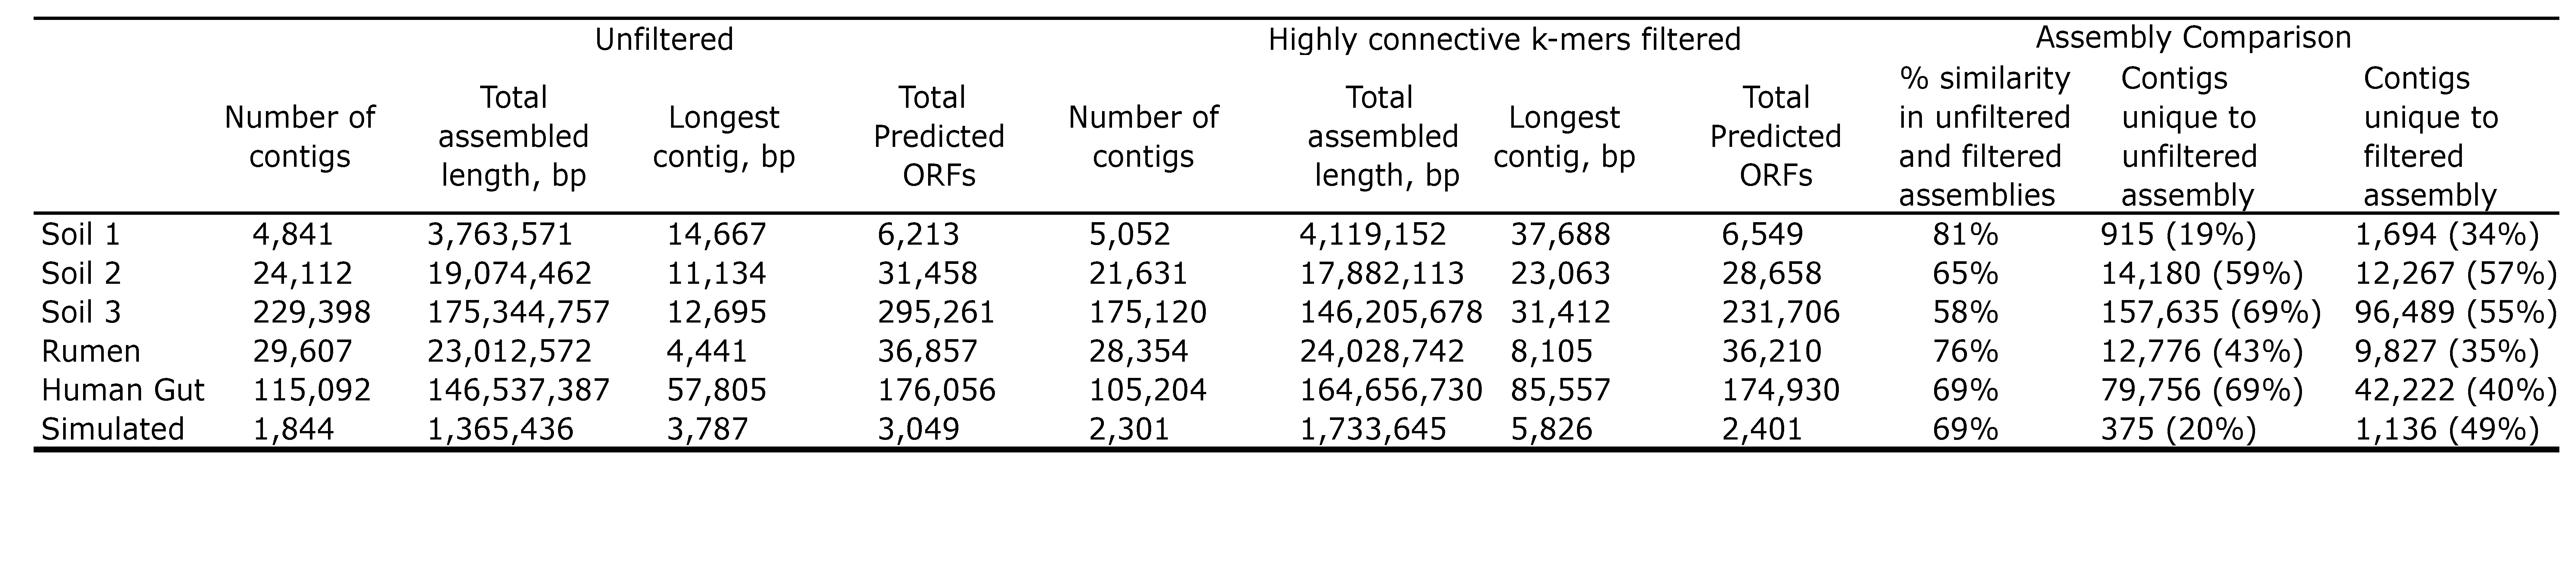
\includegraphics[width=5in]{./figures/assemblies.pdf}}
\caption{Comparison of unfiltered and filtered (removal of highly connecting k-mers) assemblies of various metagenome lumps.}
\end{figure}

\begin{figure}
\center{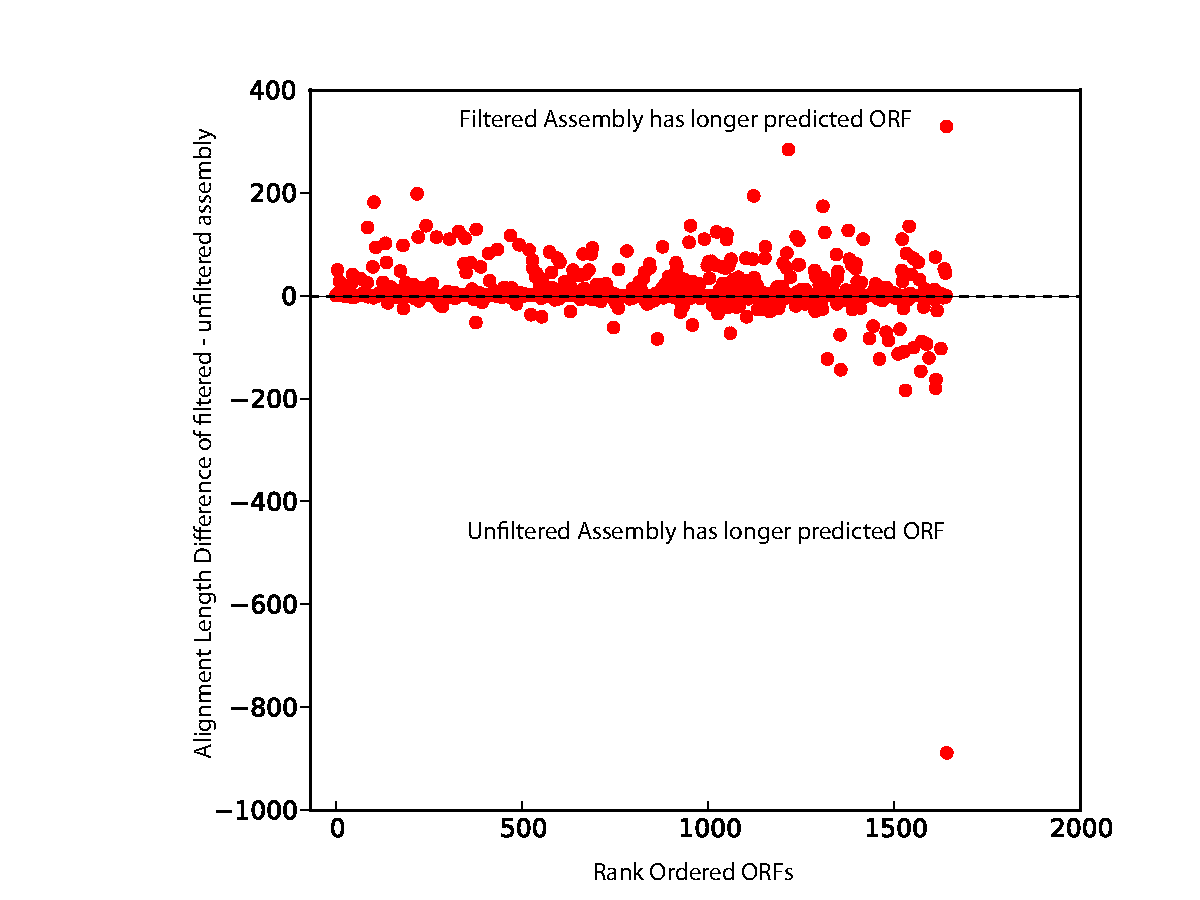
\includegraphics[width=5in]{./figures/orf_lengths.pdf}}
\caption{Alignment lengths of ORFs shared between unfiltered and filtered assemblies (removal of highly connective k-mers) of the simulated metagenome are compared.  Difference in alignment length of predicted ORFs to contigs is shown (filtered assembly - unfiltered assembly alignment length).}
\end{figure}

\subsubsection{Effects of removing highly-connecting k-mers on metagenome lumps}
Comparing the unfiltered and filtered assemblies of the rumen, human gut, and soil metagenomes, we observed that removing highly-connecting k-mers resulted in increased maximum contig lengths (ranging from 48\% to 157\%).   The effects of filtering highly-connecting k-mers on total length of assembly and number of predicted ORFs varied (Table X).   For the smallest soil, human gut, and rumen metagenomes, filtered assemblies had a longer total length.  For the soil metagenomes containign 100 million and 500 million reads, the total length of assembly decreased 6 and 17\%, respectively.  The total number of predicted ORFs decreased for filtered assemblies (ranging from 1 to 22\% fewer ORFs), with the exception of the smallest soil metagenome.  Comparing the constituent k-mers between unfiltered and filtered assemblies, we observed that the assemblies of the environmental metagenomes, like the simulated assemblies, were also quite different.  Similarity of constituent k-mers ranged from 58% to 81% for unfiltered and filtered assemblies.   A large proportion of contigs (Table X) were also unique to either the unfiltered or filtered assembly.
	We compared the assemblies of the ruman metagenomic lump to 15 draft genomes predicted from the published assembly of the full rumen metagenome \cite{Hess:2011p686}.  We compared the number of predicted ORFs from unfiltered and filtered assemblies which matched these genomes.  For the unfiltered assembly, 4,607/36,857 (12\%) predicted ORFs had a best match to the draft genomes.  The filtered assembly contained more matches to the draft genomes, 4,618/36,210 (13\%).  A total of 117 ORFs were identified in both assemblies.  Among these ORFs, 51 ORFs when aligned to draft genomes were longer in filtered assembly, 50 ORFs were longer in the unfiltered assembly, and 16 ORFs had identical alignment lengths to draft genomes.  

\section{Discussion}

\subsection{Characteristics of the lump did not appear to be biological in origin.}

We were able to separate several metagenomic assembly graphs into millions of disconnected assembly subgraphs representing sequences originating from different genomes.  The largest of these subgraphs, called the lump, contained a disproportionate number of reads relative to other subgraphs.  Initially, we considered that this lump consisted mainly of connecting sequences which were conserved across multiple genomes (i.e. 16S rRNA, ITS regions).  However, efforts to remove conserved genes from datasets did not significantly break apart the lump (data not shown).  Furthermore, the large size of the lump within metagenomic data compared to that of a simulated metagenomes (i.e., 75\% of reads in the human gut metagenome vs. 5\% in simulated) suggested that some connectivity within this lump was not biological (Table X).  Comparing soil metagenomes of increasingly larger sizes, we observed that with increasing sequencing, there was a supra-linear increase in the size of the lump and thus increase in graph connectivity (Figure X). These results combined indicated that possible spurrious connectivity was present in metagenomic lumps, and we proceeded to further analyze the connectivity these sequences.

\subsection{Position-specific biases indicate that sequencing artifacts are present in the lump.}
We first assessed the degree of connectivity within the lump by measuring the local graph density of metagenomic lumps.  For a mixture of genomes, the local graph density was measured to be low, less than 2\% of nodes with graph density greater than 20.  For the lump of connected reads of a simulated Illumina sequencing dataset of these genomes, the graph density was unsurprisingly larger with 17\% of nodes having a graph density greater than 20.   For the metagenomic lumps, however, the degree of connectivity was consistently larger than the simulated dataset, with an average of 35\% of metagenomic nodes having a graph density of greater than 20.   In addition to increased connectivity, we also observed varying local graph densities with respect to the position within a read in all metagenomes (Figure X).  This position-specific bias, not observed in the simulated dataset, clearly suggested spurrious connectivity among metagenomic sequences.  

To further explore the sources of this spurrious connectivity, we identified the highly-connecting sequences within each lump which were likely causes of the lump itself.  Similarly to the observed position-specific bias of local graph density along the read, the presence of these highly-connecting sequences also had a biased presence in locations within sequencing reads (Figure X).  Given that shotgun sequencing is randomly generated, these observed position-specific biases (both local graph density and presence of highly connecting k-mers) strongly suggested that some portion of the highly-connecting sequences are not biological and are the result of sequencing artifacts.  

\subsection{Comparing position-specific trends in various metagenomes indicates preferential attachment.}
Similar position-specific trends were observed for the local graph density and the fraction of highly-connecting sequences for all metagenomes studied (Figures X and X).  The 3'-end biases of the two largest soil metagenomes were the most pronounced.  Additionally, for these soil metagenome lumps, the size of the lumps and associated position-specific trends increased at a greater rate than the amount of sequencing, suggesting the presence of spurrious connectivity.  We suspect that this connectivity is the result of an effect referred to as "preferential attachment" \cite{Barabasi:1999p1083}. In this case, highly connecting "X" sequences in a lump recruit a number of connecting "Y" reads into the lump.  As more sequences are added, these "Y" reads, which do not necessarily have to be highly-connective, recruit more "Z" reads into the lump resulting in increasingly larger lump size.  For soil metagenomes, where sequencing coverage is relatively low and diversity is high (5.6\% coverage for the largest soil metagenome), increased sequencing would cause preferential attachment of "X", "Y", and "Z" reads resulting in increasingly larger lump sizes.  For metagenomes with less complexity, like that of the human gut and cow rumen (32.4\% and 3.5\% coverage), the number of the "Y" and "Z" reads which are lump-associated but not highly-connective would increase (because of the increased sequencing coverage) at a greater rate than than "X" reads.   This would effectively introduce a greater proportion of sequences in the lump which would not be identified as highly-connective and result in an overall decrease in the total fraction of these sequences.  Overall, we suspect a baseline 3' end presence of highly-connecting sequences which are sequencing artifacts, and the effects of these sequences on the size and connectivity of the lump depends largely on sequencing coverage.

\subsection{Removing highly-connecting sequences improves assembly overall.}
Although some of the highly-connecting sequences in metagenomic lumps are sequencing artifacts (given their position-specific bias), it is apparent that not all of these sequences are artifacts as they are also present in the error-free simulated dataset (3\% of the unique k-mers identified as highly-connective). Regardless of the origin of these sequences, we were interested in their incorporation into resulting assemblies.  For all datasets studied, we observed that these sequences were under-represented in the final assembly compared to their presence in original sequencing reads (Table X).  Moreover, when these sequences were incorporated into assembly, they tended to begin or end contigs (Figure X).  These results suggest that, overall, the assemblers are challenged by characteristics of these sequences regardless of their biological or non-biological origins and that the removal of these sequences would have little effect on the final assembly. 
	We evaluated the effects of removing these sequences with the simulated dataset.  This was an ideal case study because it contains no sequencing errors or biases and could be validated by the original reference genomes.  We compared the assembly of the simulated dataset before and after filtering out highly-connected sequences to evaluate the biological effects of these sequences on assembly.  We found that the unfiltered and filtered assemblies were quite different based on constituent k-mer composition (31% different) and the total number of unique ORFs (34\% ORFs unique to only the filtered assembly).  Overall, removal of highly-connecting sequences resulted in an overall improval of the assembly.  The filtered assembly contained 29\% more contigs and 51\% longer assembly length (for contigs greater than 500 bp) than the unfiltered assembly (Table X).  The filtered assembly also resulted in 27\% more predicted ORFs which had matches to reference genomes.  In addition to identifying more ORFs, the filtered assembly contained a greater number of equal length or longer ORFs when compared to similar ORFs in the unfiltered assembly (Figure X).  In combination, these results indicate that removing highly-connecting sequences, even if originating from real biological connectivity, improves the overall assembly.  
	Comparing soil, human gut, and rumen metagenomes, we also observed large differences in unfiltered and filtered assemblies (Table X).  The removal of highly-connecting sequences resulted in gaining new contigs and losing unfiltered contigs (Table X).  Unlike the simulated metagenome, these assemblies are more challenging to evaluate as the original source genomes are unknown.  Based on a small number of draft reference genomes which were previously validated in cite Hess, we evaluated the rumen unfiltered and filtered assemblies.  Overall, in addition to slightly more predicted ORFs overall, the filtered assembly also contained more ORFs which had improved alignments to the reference genomes.  
	
\section{Conclusion}
	We have identified the presence of sequences in metagenome datasets which are highly-connective and result in producing a large, dominant set of reads which are, at least partially, artificially  connected in metagenomic datasets.  We demonstrated that the identification and removal of these sequences in a simulated dataset results in improved assembly.  Within metagenomes, these sequences not only do not appear to be well-incorporated into assemblies.  




\section{Methods}

@Needs a good readthrough for completeness - to do

\subsection{Metagenomic datasets}

All datasets, with the exception of the agricultural soil metagenome, were from
previously published datasets. Rumen-associated sequences (Illumina)
were randomly selected from the rumen metagenome available at ftp://ftp.jgi-psf.org/pub/rnd2/Cow\_Rumen. Human-gut associated sequences (Illumina) of samples MH0001 through MH0010 were obtained from ftp://public.genomics.org.cn/BGI/gutmeta/Raw\_Reads. The agricultural
soil metagenome was from the sequencing (Illumina) of Iowa corn soil and is currently unpublished. All reads used in this study were quality-trimmed for Illumina's read segment quality control indicator, where a quality score of 2 indicates that all subsequent
regions of the sequence should not be used. After quality-trimming,
only reads with lengths greater than 30 bp were retained. All quality
trimmed reads used in this study are available at X.  The number of reads after quality-trimming is shown in Table 1 for each metagenome. The simulated high complexity, high coverage
dataset was previously published (Pignatelli, 2011).  Coverage of each metagenome was estimated by aligning trimmed sequencing reads to assembled contigs with lengths greater than 500 bp.  For coverage estimates, the assembly of each metagenome was performed using Velvet (v1.1.05) with the following parameters:  K=33, exp cov=auto, cov cutoff=0, no scaffolding.  For datasets larger than 50 million reads, metagenomes were partitioned with the methods described in (cite PNAS paper) prior to assembly to overcome computational memory limitations for assembly.  Reads were aligned to assembled contigs with Bowtie (v0.12.7), allowing for a maximum of two mismatches.  

\subsection{Lightweight, compressible de Bruijn graph representation}

We used a lightweight probabilistic de Bruijn graph representation
to explore k-mer connectivity of the assembly graph (cite PNAS paper).
The de Bruijn graph stores k-mer nodes in Bloom filters and keeps
edges between nodes implicitly, i.e. if two k-mer nodes exist with
a k-1 overlap, then there is an edge between them. Bloom filters are
a probabilistic set storage data structure with false positives but
no false negatives, thus the size of the bloom filters were selected
to be appropriate for the size of the dataset and the memory available.
For analyzing the graph connectivity of the studied datasets, we used
4 x 48e9 bit bloom filters for soil, rumen, and human gut datasets,
and 4 x 1e9 bit bloom filters for the simulated dataset. As metagenomic sequencing contains a mixture of multiple organisms, we
could exploit the biological structure of the sequencing by partitioning
the assembly graph into disconnected subgraphs that represent the
original DNA sequence components. The set of the largest number of
reads which were connected in the assembly graph is referre to above as a single, highly-connected lump. 

\subsection{Local graph density and identifying highly-connected k-mers}

We implemented a systematic traversal algorithm to highly
connected components of the assembly graph.  Waypoints were labeled to cover the graph such that they
are a minimum distance of L apart. Originating from a waypoint, all
k-mers are systematically and exhaustively traversed within a region
that is the distance N.   The local graph density was calculated as the number of X k-mers reachable within a distance N divided by the distance N.  Thus, the local graph density of a linear sequence would be 2, and additional branches or repeats would increase graph density.   To evaluate the extent of connectivity within each metagenomic lump, we calculated the number of nodes (K=32) with a local graph density of greater than 20 when N=100 and determined these nodes to be "highly dense" (Table X).  We also evaluated the degree to which graph density varied by position along a read.  For each k-mer in a read, the local graph density within N=10 nodes was calculated.  This average local graph density by k-mer position for all reads was subsequently calculated (Figure X).

@brain fart - fix highly dense - there's better phrases I'm sure

We examined the position of these highly-connective k-mers in reads contributing
to the lump. Each sequence in the lump was broken into its constituent
k-mers and evaluated to be highly-connective or not highly-connective.  The total fraction of k-mers within each dataset lump which were identified
as highly-connective and are shown in Figure X. 



\subsection{De Novo Metagenomic Assembly}
De novo metagenomic assembly reads within each metagenomic lump
were completed with Velvet (v1.1.02, cite Zerbino) with the following
parameters: velveth -short -shortPaired (if applicable to the dataset)
and velvetg -exp\_cov auto -cov\_cutoff 0 -scaffolding no.  For soil 1, soil 2, rumen, and simulated metagenomes, assemblies were performed at K=25, 27, 29, 31, and 33 and merged with Minimus (Amos v3.1.0, cite).  For soil 3 and human gut metagenomes, assemblies were performed at only K=33 due to the size of the datasets.  

To study the effects of highly connecting sequences on metagenomic assembly, these k-mers were filtered from reads by truncating the reads at the location of these sequences and the remaining reads assembled as described above.

@AC...Assemblies were also performed with ABYSS (v1.2.0, cite) with the following parameters: ABYSS -k 33  - do we want to anything with this?


\subsection{Identifying properties of highly-connecting k-mers}
The enrichment of knot-causing k-mers in unfiltered reads was studied
by identifying the fraction of unique k-mers in unfiltered sequencing
reads and in their resulting assembled contigs. The ratio of these k-mer fractions (unfiltered reads/assembled contigs) estimates the enrichment of knot-causing k-mers in the reads. 

To further understand the contribution of the knot-containing
contigs to unfiltered and filtered assembly differences, we calculated
the difference in constituent unique k-mers between knot-containing
contigs and the filtered contigs (resulting from assembly of knot-filtered reads)
using Bloom filters as described above. The fraction of total knot-causing
k-mers between the two assemblies was calculated by dividing the number
of different k-mers in knot-containing contigs by the total number
of different k-mers in unfiltered and filtered contigs. 

The location of knots in unfiltered contigs was also studied. Contigs containing
knot-causing k-mers were divided into 100 equally-sized regions. For
each contig, the total number of knot-causing k-mers and total number
of k-mers was calculated. For each dataset, the total fraction of
knot-causing k-mers in each region for all contigs was calculated
and is shown in Figure X.

The presence of knot-causing k-mers in ORFs was examined. Fraggenescan
(v1.1.15, cite) with the following parameters: -complete=0 -training=454\_10
was used to identify ORFs in unfiltered contigs. We defined the "edge''
of an ORF within a contig to be between 32 bp (k-mer size used in
our de Bruijn graph representation) outside of of an ORF to within
16 bp (k/2) inside the ORF. The remaining internal ORF bases were
defined as inside the ORF, and external bases were defined as outside
the ORF. For each base within a contig, we determined if it was the
initial base of a knot causing k-mer and if it was located inside, outside,
or at the edge of an ORF. The distribution of knot-causing bases (k-mers)
between the inside, outside, and edge were then compared to the total
distribution of all bases. 

To evaluate assemblies of the simulated and rumen datasets, ORFs and contigs were aligned to the original 112 genomes used to generate the simulated metagenome and 15 draft rumen genomes  \cite{Hess:2011p686} using BLAST (v2.2.25).  For specific contig regions (the ORFs which were edge-enriched for knot-containing sequences), mismatches between assembled sequences and reference genomes were identified to evaluate the accuracy of assembly.  To determine the effects of removing highly-connecting sequences, the alignment lengths of contigs from unfiltered and knot-filtered assemblies which shared identical top blast alignments were compared.    

\subsection{Comparison of shared constituent k-mers}

To calculate the number of shared unique k-mers between assembly A and assembly B, constituent k-mers of contigs from assembly A were loaded into bloom filters (4 x 1e9 bits). Subsequently, the constituent k-mers from the assembly B were queried against
the assembly A k-mers. The number of shared unique k-mers is
dependent on which assembly is initially loaded into the bloom filters. Thus, each comparison was completed twice, once with the unfiltered
assembly and once with the filtered assembly initially loaded into the bloom
filter. Assembly similarity was determined by the lowest fraction
of shared unique k-mers between these two comparisons (Figure X). 

@Need to add in vector assembly comparisons - not sure how this is done well enough to write about it, vector blah blah

\section{Conclusion}
Removing these lumps is computationally very useful, enabling MetaIDBA as well as scaling approaches

\bibliography{artifacts-paper-bib}
\bibliographystyle{plain}


\end{document}